%==============================================================================
% Sjabloon onderzoeksvoorstel bachelorproef
%==============================================================================
% Gebaseerd op LaTeX-sjabloon ‘Stylish Article’ (zie voorstel.cls)
% Auteur: Jens Buysse, Bert Van Vreckem

\documentclass[fleqn,10pt]{voorstel}

%------------------------------------------------------------------------------
% Metadata over het voorstel
%------------------------------------------------------------------------------

\JournalInfo{HoGent Bedrijf en Organisatie}
\Archive{Bachelorproef 2018 - 2019} % Of: Onderzoekstechnieken

%---------- Titel & auteur ----------------------------------------------------

% TODO: geef werktitel van je eigen voorstel op
\PaperTitle{Is Python een toegevoegde waarde om uitgebreid aan te leren in het hoger onderwijs?}
\PaperType{Onderzoeksvoorstel Bachelorproef} % Type document

% TODO: vul je eigen naam in als auteur, geef ook je emailadres mee!
\Authors{Jorik Spiesschaert\textsuperscript{1}} % Authors
\CoPromotor{TBA\textsuperscript{2} (Bedrijfsnaam)}
\affiliation{\textbf{Contact:}
  \textsuperscript{1} \href{mailto:jorik.spiesschaert.y9481@student.hogent.be}{jorik.spiesschaert.y9481@student.hogent.be};
}

%---------- Abstract ----------------------------------------------------------

\Abstract{
Door een merkwaardige groei van Python zien we meer en meer dat deze programmeertaal wordt geimplementeerd in veel deeldomeinen van de informatica. Maar wordt hier wel voldoende aandacht besteedt aan deze taal op de schoolbanken? In dit onderzoek wordt er getoetst ofdat de kennis van Python bij schoolverlaters wel voldoende is wanneer ze het werkveld betreden. Er wordt verwacht dat de kennis onvoldoende groot is, en dat Hogescholen meer aandacht moeten besteden aan Python, dat een opmerkelijke evolutie doorgaat. 

}

%---------- Onderzoeksdomein en sleutelwoorden --------------------------------
% TODO: Sleutelwoorden:
%
% Het eerste sleutelwoord beschrijft het onderzoeksdomein. Je kan kiezen uit
% deze lijst:
%
% - Mobiele applicatieontwikkeling
% - Webapplicatieontwikkeling
% - Applicatieontwikkeling (andere)
% - Systeembeheer
% - Netwerkbeheer
% - Mainframe
% - E-business
% - Databanken en big data
% - Machineleertechnieken en kunstmatige intelligentie
% - Andere (specifieer)
%
% De andere sleutelwoorden zijn vrij te kiezen

\Keywords{Onderwijs. Python --- Scripting } % Keywords
\newcommand{\keywordname}{Sleutelwoorden} % Defines the keywords heading name

%---------- Titel, inhoud -----------------------------------------------------

\begin{document}

\flushbottom % Makes all text pages the same height
\maketitle % Print the title and abstract box
\tableofcontents % Print the contents section
\thispagestyle{empty} % Removes page numbering from the first page

%------------------------------------------------------------------------------
% Hoofdtekst
%------------------------------------------------------------------------------

% De hoofdtekst van het voorstel zit in een apart bestand, zodat het makkelijk
% kan opgenomen worden in de bijlagen van de bachelorproef zelf.
%---------- Inleiding ---------------------------------------------------------

\section{Introductie} % The \section*{} command stops section numbering
\label{sec:introductie}

Wanneer het management in het bedrijf een strategische of tactische beslissing wil maken, is deze beslissing gebaseerd op data afkomstig uit verschillende databronnen. Daarom is er bij grote ondernemingen (en tegenwoordig ook bij KMO’s) nood aan een rapporteringssysteem. Voor het opstellen en onderhouden van datawarehouses wordt een bepaald budget voorzien. Relaties leggen tussen verschillende data is dan ook een grote uitdaging. Daarom is het dus belangrijk dat het model op de juiste manier ontworpen wordt om kosten te beperken wanneer men de datawarehouse wil onderhouden/uitbreiden. Hiervoor bestaan verschillende modelleertechnieken. In dit onderzoek worden enkel het Kimball dimensioneel modelleren en Data Vault 2.0 vergeleken. We proberen in dit onderzoek de volgende vraag te beantwoorden: \textbf{Waar zitten de verschillen bij het modelleren met Data Vault 2.0 en het dimensioneel modelleren?}

Ook zal er een antwoord trachten gevonden te worden op volgende deelvragen:

\begin{itemize}
	\item Zijn er verschillende manieren van aanpak mogelijk?
	\item Hoe flexibel/schaalbaar zijn beide systemen?
	\item Is er een verschil in performantie?
	\item Hoe verschillen de technieken naar onderhoud toe?
\end{itemize}

Bij DHL Pharma Logistics gebeurt het berekenen van de KPI's (Key Performance Indicators) nog altijd manueel. Zo worden de KPI's berekend via een rekenmachine en handmatig ingevoerd in een Excel-bestand. De informatie die nodig is om verschillende berekeningen te maken is afkomstig uit verschillende databronnen (mainframe, Cronos, Excel-sheets, ..). Dit neemt veel tijd in beslag, dus beslist de firma om een deel van de KPI's te automatiseren. Hiervoor zal een datawarehouse moeten opgezet worden. Deze zal gemodelleerd worden in Data Vault 2.0. Maar is dit wel de beste oplossing? Dit onderzoek zal uitwijzen of Data Vault 2.0 wel degelijk de beste oplossing is.
%---------- Stand van zaken ---------------------------------------------------

\section{Literatuurstudie}
\label{sec:state-of-the-art}
\subsection{Data Vault 2.0}
\subsubsection{Architectuur}
De architectuur van Data vault bestaat voornamelijk uit 3 lagen: De staging area, de raw data vault area en de Business vault. De staging area wordt gebruikt om alle data tijdelijk te stockeren. Deze wordt opgeslagen in de architectuur van het bronsysteem. Daarna wordt de data doorgezonden naar de volgende laag: de raw data vault. Hierbij wordt de architectuur omgevormd naar een data vault. Hierop worden dan data manipulaties gemaakt en wordt de data doorgezonden naar de volgende laag, de business vault. Data marts worden gecreëerd op de business vault \autocite{Linstedt2015}.

\begin{figure}[h]
	\centering
	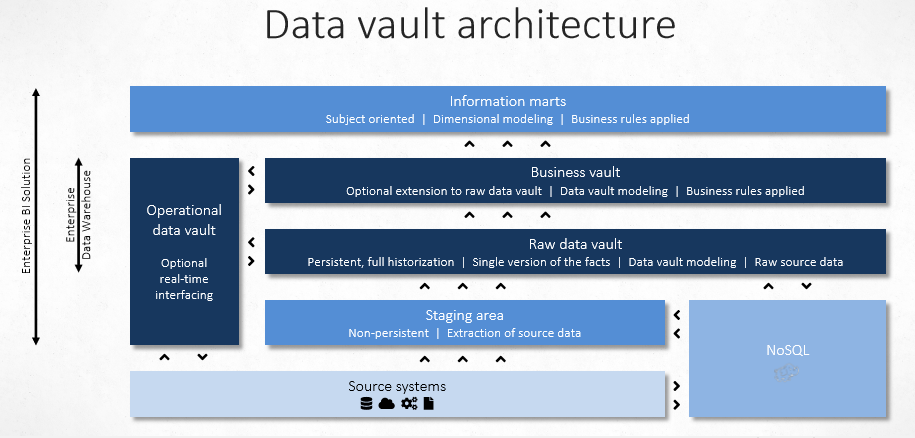
\includegraphics[scale=0.345]{images/DVArchitectuur.png}
	\caption{Data Vault architectuur voorgesteld door \textcite{Stroobants2018}.}
	\label{fig:dvarch}
\end{figure}

\subsubsection{Entiteittype's}
Bij data vault wordt er een onderscheid gemaakt tussen 3 verschillende entiteiten: hub, link en satelliet. In een hub wordt een hash sleutel opgeslagen die gebaseerd is op de identifier van die entiteit en metadata (zoals de bron en wanneer de record is ingevoerd). Een link is entiteit die verantwoordelijk is om verschillende hubs met elkaar te verbinden. Hierin worden de hash sleutels van de verbonden entiteiten in opgeslagen. Satellieten kunnen verbonden worden met hubs en links. Deze bevatten de inhoudelijke data van de entiteit.  

\subsection{Dimensioneel modelleren}
\subsubsection{Architectuur}
Bij het dimensioneel modelleren via Kimbell is er 1 enkele laag, hierin worden alle operaties uitgevoerd (ETL: Extraction, Transaction en Load). De data wordt ingeladen in een ster-schema. Op deze laag worden dan data marts gebouwd. \autocite{Jukic2006}

\subsubsection{Entiteittype's}
Bij deze techniek bestaan er 2 entiteittype's: feit tabellen en dimensionele tabellen. De feit tabellen bevatten alle transactionele data, data waarop je eigenlijk berekeningen kan maken. Dimensionele tabellen bevatten meer informatie over de transactionele data.

% Voor literatuurverwijzingen zijn er twee belangrijke commando's:
% \autocite{KEY} => (Auteur, jaartal) Gebruik dit als de naam van de auteur
%   geen onderdeel is van de zin.
% \textcite{KEY} => Auteur (jaartal)  Gebruik dit als de auteursnaam wel een
%   functie heeft in de zin (bv. ``Uit onderzoek door Doll & Hill (1954) bleek
%   ...'')


%---------- Methodologie ------------------------------------------------------
\section{Methodologie}
\label{sec:methodologie}
Voor dit onderzoek zullen er twee datawarehouses opgezet worden in een SAP HANA-omgeving. De eerste datawarehouse zal gemodelleerd worden in Data Vault 2.0, de andere in een dimensioneel model. De SAP HANA omgeving is 'on-premise' die draait in een Microsoft Azure omgeving. Het modelleren zal deels gebeuren in Eclipse (die een remote-verbinding maakt met Azure) en deels via een web IDE voor HANA (Xsengine). Wanneer beide datawarehouses operationeel zijn, kan er gestart worden met de vergelijking. De datawarehouses zullen gebaseerd zijn op KPI's die gedefinieerd zijn bij DHL Pharma Logistics.

\subsection{Performatie}
Om de performantie van beide systemen te vergelijken, zullen er een aantal verschillende queries uitgevoerd worden op data marts gebaseerd op deze datawarehouses. Op basis van uitvoeringstijd kunnen we deze dan met elkaar vergelijken. Zo kunnen we te weten komen of er wel degelijk een verschil is tussen beide architecturen in performantie en hoe groot de verschillen zijn. 

\subsection{Audit}
Stel dat er op 2 verschillende databronnen klantengegevens opgeslagen wordt, zal er een keuze moeten gemaakt worden. Van welke bron haal ik mijn gegevens? Indien er verschillende problemen optreden met data, willen we graag kunnen onderzoeken waar het probleem zich heeft voorgedaan. Hiervoor voegen we META-data toe aan de data die ons verteld waar en wanneer de data werd opgehaald. 

\subsection{Schaalbaarheid}
Hoe wordt er omgegaan met grote hoeveelheden data in beide architecturen? Merken we hier een significant verschil? Zien we de uitvoeringstijden lineair/exponentieel stijgen? 

\subsection{Flexibiliteit}
De vereisten voor rapportering verandert vaak bij bedrijven. Soms moeten KPI's worden toegevoegd, soms moeten deze gewijzigd worden. Maar wat als er databronnen in het bedrijfsnetwerk toegevoegd? Hoe gemakkelijk kunnen deze wijzigingen gemaakt worden in beide architecturen? Dit zullen we onderzoeken door een nieuwe KPI toe te voegen aan het systeem. 
 


%---------- Verwachte resultaten ----------------------------------------------
\section{Verwachte resultaten}
\label{sec:verwachte_resultaten}

Op basis van het uitgevoerde onderzoek zullen we hiervan een resultaat kunnen opstellen. Ik verwacht dat beide technieken zijn voordelen en nadelen zullen hebben. Zo zal Data Vault 2.0 een modelleertechniek zijn die zeer flexibel is, maar dit zal ten koste gaan van de performantie. Het dimensionele model zal zo performanter zijn, maar weinig flexibiliteit bieden.

%---------- Verwachte conclusies ----------------------------------------------
\section{Verwachte conclusies}
\label{sec:verwachte_conclusies}

Aangezien Data Vault 2.0 veel flexibiliteit te bieden heeft, zal dit de beste oplossing zijn wanneer alle data verspreidt staat op verschillende systemen. Bij Data Vault 2.0 is het namelijk mogelijk gemakkelijk nieuwe databronnen toe te voegen in een datawarehouse. Maar wanneer men de de data marts wil ontwerpen, zal men nog steeds moeten gebruik maken van dimensioneel modelleren. Wanneer een bedrijf weinig databronnen heeft en deze weinig veranderen, is dimensioneel modelleren de betere oplossing. 

Voor DHL Pharma Logistics zal Data Vault 2.0 dan ook de beste oplossing zijn, aangezien hun data verspreidt staat over enkele systemen. Zo kunnen ze hun KPI's ook nog beter definiëren en makkelijker aanpassen in het systeem. 


%------------------------------------------------------------------------------
% Referentielijst
%------------------------------------------------------------------------------
% TODO: de gerefereerde werken moeten in BibTeX-bestand ``voorstel.bib''
% voorkomen. Gebruik JabRef om je bibliografie bij te houden en vergeet niet
% om compatibiliteit met Biber/BibLaTeX aan te zetten (File > Switch to
% BibLaTeX mode)

\phantomsection
\printbibliography[heading=bibintoc]

\end{document}
